\documentclass[exercice]{thedocument}%
\startdatakeys
\source{}
\cycle{}
\competencesDuSocle{}
\connaissancesRequises{}
\competencesTravaillees{}
\enddatakeys
\begin{document}%
    \begin{enumerate}
        \begin{minipage}[t]{.5\linewidth}
            \item Reproduire à main levée une figure analogue à la figure suivante.
        \end{minipage}\hspace{.01\linewidth}
        \begin{minipage}[t]{.48\linewidth}
            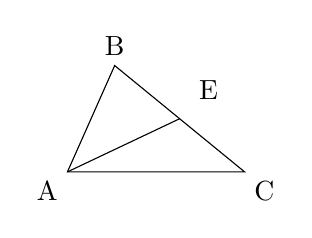
\begin{tikzpicture}[scale=0.75]
                \coordinate[label=below left:A](A)at(0,0);
                \coordinate[label=below right:C](B)at(3,0);
                \coordinate[label=above:B](C)at(0.8,1.8);
                \path(B)--(C)coordinate[pos=0.5](E);
                \node[label=above right:E]at(E){$ $};
                \draw(A)--(B)--(C)--cycle;
                \draw(A)--(E);
            \end{tikzpicture}
        \end{minipage}
        \item Coder sur la figure les angles $\widehat{\mathspoint{ABC}}$ par (1),
        $\widehat{\mathspoint{AEC}}$ par (2) et $\widehat{\mathspoint{ECA}}$ par (3).
    \end{enumerate}
\end{document}
